\documentclass[letterpaper,12pt,landscape,twocolumn]{book}
\usepackage[margin=0.5in,pass]{geometry}
\usepackage{xcolor}
\usepackage{hyperref}
\hypersetup{
  colorlinks,
  linkcolor={blue!50!black},
  citecolor={blue!50!black},
  urlcolor={blue!50!black}
}
\usepackage{graphicx}
\usepackage{ragged2e}
\usepackage{tabularx}

\title{\Huge \textbf{Springers} \\ \Large A Roleplaying Game For the Multiverse }
% Author
\author{ \textbf{by Dan Noland} \\ \textbf{For The 2015 RPG Geek 24-Hour RPG Contest}}
\begin{document}
\RaggedRight
\frontmatter
\maketitle

\let\cleardoublepage\clearpage

\tableofcontents
\mainmatter
%%%%%%%%%%%%%%%%
% CHAPTER 0    %
%%%%%%%%%%%%%%%%
\chapter{What Is This?}
\section{Role-Playing Games}
Springers is a tabletop role-playing game (often abbreviated RPG). As
the name suggests this is a game where you gather with your friends
and take on the roles of characters to tell a story together and enjoy
one another's company. The input from your friends and some chance
outcomes from dice will take the story in directions you didn't
expect. 

There are lots of different types of role-playing games just as there
are lots of different types of board games or sports. Some
role-playing games focus on sword \& sorcery fantasy stories or
espionage stories in a dark cyberpunk future or tales of romance and
courtship. For almost any genre of book, film, or television you can
imagine there is a corresponding role-playing game where you can 
inhabit characters from that genre and tell those stories with your
friends. 

Lots of ink has been spilled describing RPGs to new players, but lots
of habits and game etiquette are picked up by playing with friends
and acquaintances. Often an example of play helps. Here are some
resources for those that are new to the hobby.

\begin{itemize}
\item Learn to Play Tabletop RPGs - A site with advice and intro
  videos for new players -
  \href{http://learntabletoprpgs.com/}{http://learntabletoprpgs.com/} 
\item TableTop - Wil Wheaton and other minor celebrities gather to
  play tabletop games together. Their series on the game ``Fiasco''
  perfectly captures how RPGS are played -
  \href{https://www.youtube.com/watch?v=uuJizhyf-y4}{Fiasco Set-Up},  
  \href{https://www.youtube.com/watch?v=WXJxQ0NbFtk}{Fiasco Play Part One},  
  and \href{https://www.youtube.com/watch?v=Aj7NcdDh-WM}{Fiasco
    Play Part Two}  
\item The Walking Eye Podcast - Listen to their cast play lots of
  different games together - \href{http://www.thewalkingeye.com/}{http://www.thewalkingeye.com/} 
\item The RPG subreddit beginner's guide - An introductory wiki
  maintained by the community - \href{https://www.reddit.com/r/rpg/wiki/beginnersguide}{https://www.reddit.com/r/rpg/wiki/beginnersguide} 
\end{itemize}

\subsection{So What Kind of Role-Playing Game is This?}
In Springers each player will take on the role of a disembodied mind
jumping randomly through an infinity of possible universes. Each time
you play your disembodied mind will find itself temporarily
ppossessing the body of someone who normally lives in that universe. You
work to solve their problems and then your mind leaves their bodies,
hopefully with them better off than before, and travels on to the next
universe. 
\newline
We've all seen
\href{https://en.wikipedia.org/wiki/Quantum_Leap}{Quantum Leap} right?
It's like that.   

\section{What Do I Need In Order to Play?}
To play Springers each player will need two ten sided dice (2d10),
paper, and pencil. In addition one deck of standard playing cards is
needed. It can be shared among the group. Also a stack of 3x5 index
cards will come in handy.

\chapter{A Springer's Guide to the Multiverse}

\section{Wait, So What Kind of Character is This?}

You play a ``Springer'' a rare being who's mind jumps from one universe to
another. In fact you could say a Springer is nothing but a mind. They don't
seem to have a bodies of their own. When their mind jumps to a new world
it needs to inhabit the body of some conscious intelligent being in
order to perceive and interact with the universe. 

Some believe that
seeking intelligent minds is how Springers unconsciously navigate the
multiverse. It prevents them from ending up in any of the infinite
number of universes that contain nothing but hard vacuum and gamma
radiation. Fortunately for Springers there are also an infinite number
of universes where intelligent life exists. 

No one truly understands the process of being ``inhabited'' or
``possessed'' by a Springer. What is certain is that when the pattern
of the Springer's mind is laid down atop the existing brain (or
whatever structure intelligent beings in this universe use to think)
the mind and consciousness of that being is temporarily
suppressed for as long as the Springer remains. This results in a
period of temporary amnesia that the being will have difficulty
explaining afterward. 

From the point of view of the Springer inhabiting a new body is only
somewhat better. They cannot direct their travels through the
multiverse or choose who they inhabit. As they leave one body there is
a sensation of falling and a white light rapidly sweeps over their
vision from the periphery until it fills their entire field of
view. Then suddenly sensation pours back in as they find themselves in
a new body. Because this happens at a seemingly random instant in the
being's life it can easily be awkward or dangerous. Whatever they were
doing the moment before the Springer jumped into their mind is exactly
the situation that the Springer now finds itself facing. Game masters
are encouraged to make liberal use of \textit{in medias res}.

As minutes and hours pass in the new body the Springer can often
concentrate on interrogating the brain's contents to access some
rudimentary biographical information about the being they now appear
to be.

Only the Springer's mind travels between various worlds nothing
physical can possibly make the jump. 

Some mysteries that will be explored in play are: Where the Springers come
from and how they come to be. What is their place and function is in
the multiverse? Each individual Springer begins play with memories of
many past jumps, but no clear notion of where they come from or what
their destiny is. Many have ideas and even firmly held beliefs, but
none are sure. Some say that Springers are dreamers or astral
projectors that have come untethered from their original body and
must make this journey until they can find their way back to their own
bodies. Others say that Springers are a type of angel or immune system
for the universe destined to travel forever through the multiverse
correcting problems and righting wrongs. Another hypothesis states
that they are a type of self aware information from the higher realm
of mathematics. Still others say that Springers are cursed and need to
atone for misdeeds in a previous life or that something has gone wrong
with their reincarnation. Any or none of these could be true. Your
group will work to find your own answers to these questions.

\section{What is the Collective Noun for a Group of Springers?}

Traveling through the multiverse by endlessly hopping from one strange
body to another is a draining and lonely existence. However some
Springers are able to travel as a group. How this is possible is as
poorly understood as the nature of the jumping itself. Perhaps they
travel together as part of God's plan or because of quantum
entanglement between their information matrices or because because
their souls carry the memory of unresolved issues between them.

In any case the Springers bound together in such a group typically use
a term invented by the author Kurt Vonnegut in several universes
including the one containing Earth-262144. That author defined a \textit{karass}
as ``a team that does God's Will without ever discovering what they
are doing.'' 

Springers are always able to recognize one another despite their ever
shifting series of host bodies. There is a certain familiarity to the
presence of any Springer in your \textit{karass} that can be sensed at
a moderate range (across a room, but not across a sports stadium). 

There are malicious Springers roaming the
multiverse, terrible minds that have given in to insanity or
sadism. Your \textit{karass} may encounter one or even many traveling
in a \textit{diabolic karass}. However all players are expected to
take on the roles of well meaning Springers that treat the lives of
the beings who's bodies they temporarily inhabit with respect. This
does not mean that they cannot be cynical or flawed characters. 

\section{The Multiverse}

What is in the multiverse you ask? Well it contains every possible
type of place you can imagine and also an infinite number of
places that you cannot imagine. Every historical version of earth
every and every alternate history where something went slightly
differently are all potential landing spots for Springers.

In some universes the rules of physics work quite differently. For
instance in a number of universes the fine-structure constant is just
right to allow telepathic communication between brains via
electromagnetism. In other universes the luminiferous {\ae}ther has
the correct resonance to allow the working of magical effects. 

Creativity and variety in universes is strongly encouraged. Certainly
all the universes in film, comics, literature, and television are
available. But it can be rewarding to occasionally create a truly
alien universe.

\chapter{Character Creation}

\section{Attributes}
Springers have four mental attributes that follow them throughout the
multiverse. They are:

\begin{itemize}
\item \textbf{Quick Thinking} : The ability to think on your feet, when under
  fire, or to react quickly.
\item \textbf{Empathy} : The ability to interact with other minds
  effectively. To understand their thinking and act appropriately. 
\item \textbf{Reasoning} : The ability to deduce a result from first
  principles, abstract and critical thinking. 
\item \textbf{Cool} : Mental distance from the present situation and
  self assurance. The ability to remove yourself from your own
  emotions and the emotions of others.
\end{itemize}

In the game we measure these attributes on a five point scale from -2
to +2. According to the following scale.

\begin{itemize}
\item \textbf{-2, Feeble} : The character has a serious deficit in
  this area and will struggle to succeed in it.
\item \textbf{-1, Poor} : The character is below average in this
  area.
\item \textbf{0, Average} : The character is about average in this area.
\item \textbf{+1, Good} : The character is above average in this
  area.
\item \textbf{+2, Great} : The character is exceptional in this
  area. Few match them. 
\end{itemize}

When building your character you may assign skills anywhere on this
scale so long as the following rules are obeyed. 

\begin{itemize}
\item \textbf{Quick Thinking} must be the mathematical negation of \textbf{Reasoning}.
\item \textbf{Empathy} must be the mathematical negation of \textbf{Cool}.
\end{itemize}

This means that if a character has a \textbf{Quick Thinking of +2}
they must also have a \textbf{Reasoning of -2}. And likewise if the
character has an \textbf{Empathy of 0} they must also have a
\textbf{Cool of 0}.

\section{Descriptors}

Choose a positive personality trait. This is who your Springer
believes themselves to be. They would list it among their virtues if
asked to account for themselves.

Choose a negative personality trait. This is who your Springer is on a
bad day. They may or may not recognize this as a flaw in themselves,
but it surely is.

Choose a gender. This has no bearing whatsoever on the biological sex
of the bodies you will inhabit, but some minds traveling the multiverse
think of themselves as female and some think of themselves as male.
Others don't feel a pull toward either gender and some have a more
dynamic notion of gender. 

That's it character creation is done. 

\section{Bonds}

Choose any number of characters in your \textit{karass}. Work with
them to describe a situation where they strongly affected your
character. Good examples: Describe a time they helped you out of a
tough spot, Describe the first time they appeared in your
\textit{karass}, Describe a time they betrayed you or let you down
that you haven't forgiven them for.

For each player with whom you create a story make a note and add a
bond to your character sheet.

\section{Wait! Aren't you Forgetting Something?}

Yes. In any given world the character will have physical attributes
appropriate to the body they happen to inhabit. Those will be part of
the physical overlay that you add to your character with each
jump. These will change each time.

More in section TODO REFERENCE.

\chapter{Playing the Game}

\section{Initial Setup}

Once everyone has built their characters the players draw cards
to see who gets to take on the role of Game Master (GM) first. High
card wins, identical face values are resolved in bridge suit order
($\spadesuit$ is better than $\heartsuit$ is better than
$\diamondsuit$ is better than $\clubsuit$). It is important to record
everyone's order in the draw. Write it down and email it to yourself
or take a photo with your phone. This will be the order you each play
as GM. 
When you are finished shuffle the cards back into the deck.

\section{Being The Game Master}

The Game Master is a special player that describes the environment
faced by the other players and all the strange and interesting people
in it. 

When it is your turn as GM you will not be playing as your usual
character. You will be busy creating problems for the other players to
resolve and portraying the beings in the little corner of the
multiverse their characters find themselves in.

The player who is GM has a few primary objectives. 

\begin{itemize}
\item \textbf{Make the Character's Lives Interesting} : Jumping from
  one universe to another should never feel like a leisurely walk in
  the park. Give them drama and action.
\item \textbf{Make The Multiverse Strange} : Everything that is
  possible, and quite a bit that isn't is going on out there. Give
  the other players something truly strange.
\item \textbf{Keep The Story Human} : The problems the characters
  face need to be relatable on some level. Even as things get
  strange always show interest in the GMPCs you portray. What do
  they hope for? Who do they love? Who do they want to impress?
\end{itemize}

If it is your turn to GM next draw a card from the deck and consult
the table below to determine what kind of problem the players will be
facing. Reveal your card to the other players. \\

\begin{tabularx}{0.45\textwidth}{p{1cm}|X}
  \textbf{$\spadesuit$} & The problem involves force or
  violence. \\ \hline
  \textbf{$\heartsuit$} & The problem involves emotion and the
  relationship between two or more beings. \\ \hline
  \textbf{$\diamondsuit$} & The problem involves a significant
  object. \\ \hline
  \textbf{$\clubsuit$} & The problem involves hidden knowledge. \\ %\hline
\end{tabularx}
\\
If this sparks an idea in you immediately, great! Otherwise ask the
players what kind of world might have this kind of problem. What kind
of beings live there? What factions might be at play? Brainstorm
with them and collect the best ideas in quick notes for the play
session. 

If the card drawn is a face-card then this session will provide clues
to the nature or destiny of the Springers or their adversaries. These
sessions advance the mythology of the Springers. When a
non-face-card is drawn it is a normal episodic sessions. 

Now draw a second card and keep it hidden from the other players. 

\begin{tabularx}{0.45\textwidth}{p{1cm}|X}
  \textbf{$\spadesuit$} & This problem is amenable to force or violence. \\ \hline
  \textbf{$\heartsuit$} & The problem may be solved by emotional
  appeal or negotiation. \\ \hline
  \textbf{$\diamondsuit$} & The situation can be improved via
  infiltration, stealth, or espionage. \\ \hline
  \textbf{$\clubsuit$} & The problem can be addressed through
  investigation, research, or magic. \\ %\hline
\end{tabularx}

\subsection{Creating Physical Overlays}

To create physical overlays for the other characters you need to
follow a few easy steps. Get out some 3x5 cards or some scratch
paper. You will need one for each player excluding yourself. 

Also do this part on your own.

\subsubsection{Descriptive Tag}

What kind of being is this? Keep it very simple. Just something to
give the players an idea. Often 2-3 words are sufficient. Some examples
some descriptive tags might be: \textit{Space Marine, Marie
  Antoinette, Reptilian Infiltrator, Crime-fighting Pop Star, Mouse
  Knight, or Clone Number 23456908} 

If you have some idea about the background of this being that is
great, because it is likely that players will want to investigate this
body their characters find themselves inhabiting.

\subsubsection{Biological Sex}
Does the being in question have a meaningful biological sex? If so
note it here also. 

\subsubsection{Physical Attributes}

You need to assign three physical attributes to each being. They are:

\begin{itemize}
\item \textbf{Body} : The strength and toughness of this body. The
  creature has wound levels equal to 3 plus, or minus, its Body rating.
\item \textbf{Agility} : The grace and speed that this body is capable
  of. 
\item \textbf{Strange} : This body's ability to interact with the
  strange physics of this place. It is used to measure aptitude with
  any odd powers that may be native to this universe. This score may
  often be given a value of N/A if the being doesn't have any powers
  or the universe in question appears to strictly follow our own
  physics.  
\end{itemize}

These attributes are rated just as the others are -2 to +2 some
exceptional beings might even have physical attributes greater than
+2. 

These values do not need to be balanced against one another as the
mental attributes do. Feel free to assign whatever stats you feel best
captures the physical nature of this being. 

There is no need to ``balance'' the physical attributes between each
3x5 card. Some beings are vastly more physically powerful than
others. That is fine. Or on a planet populated entirely by identical
clones you could give everyone the same physical attributes. This is
fine as well.

\subsubsection{Notes on Strangeness}
If this being has any strange powers make a quick note of them
here. Describe the superpowers available in a universe with
superheros. Make a note if magic is available. If everyone on the
planet has a natural telepathy make a note for the players. 

~ \\

Once you have completed those four steps for each 3x5 card put them in
a pile face down and shuffle them. Allow the players to each pick one
of the physical overlays you have created at random. That will be the
physical body they will inhabit for this session.  

\subsection{GM Advice}

As the characters move through the session working toward the
solution to the problem be sure to advantage those players that are
using the preferred method, based on your earlier secret card draw, to
solve it. This does not mean that other methods of approaching the
problem will not work, merely that one is best. You should never
insist that they use your solution to the exclusion of all others.

You should show signs of the problem the players are meant to solve
early. 

TODO: More on GM moves, when exactly to call for rolls, how to keep
the story going, in medias res, throw them into awkward situations
(e.g. opposite sides: make some Montagues and some Capulets), more
scenario building advice, etc.

\section{Being a Normal Player}

At any given time most of you won't be playing as the game
master. Instead you will be portraying your characters. 

At the beginning of the session the GM will show you a card indicating
what type of problem you are facing. He or she may also brainstorm
with you asking about they types of universes that are a good match
for that type of problem and your interests. Help them out if you have
any ideas.

The GM will also draw a secret card that lets them know which types of
approaches to the problem will be most fruitful, so be sure to try
more than one strategy for solving the problem.

You will then select one of the physical overlays the GM has prepared
at random from the pile. Look it over and see what kind of being you
have become.

The GM will then describe the situation your characters find
themselves in as they snap into consciousness in their new
bodies. Describe what you do to the GM and he or she will tell you
what happens or ask you to roll some dice.

\subsection{Conflict and Resolution}

As you move through the world looking to solve the problem you will
eventually come into conflict with someone or end up in a situation
where the outcome of your actions is uncertain. In these cases the
game master will often ask you to roll to determine the outcome. 

Rolls are always made using two ten-sided dice (2d10) often you will
have a bonus, or penalty, from your attributes. Rolls of 9 or lower
are a complete miss. Rolls between 10 and 15 inclusive are partial
success, you may get the outcome you want at a cost or have to make a
tough decision. Rolls of 16 to 19 are a Hit. On rolls of 20 or above
you not only succeed, but you and the other players decide on some way
the success gives you future advantage. 

\begin{tabularx}{0.45\textwidth}{p{2cm}|X}
  \textbf{Roll} & \textbf{Result} \\ \hline
  2-9 & Miss \\ \hline
  10-15 & Partial Success \\ \hline
  16-19 & Hit \\ \hline
  20+ & Hit \& Advantage \\ 
\end{tabularx}
\\
The GM will tell you what attribute(s) you should add to your
roll based on the type of conflict. Some common rolls are below.

When you \textbf{search the memories of your host body}
roll+\textbf{Empathy}+\textbf{Reasoning}. On a Partial Success the GM
will give you some impressions of the being's life. On a Hit the GM
will also allow you to ask two specific questions. 

When you \textbf{seek to avoid detection}
roll+\textbf{Reasoning}+\textbf{Agility}. On a Hit you pass
unnoticed. On a partial success you make a small mistake. The GM will
offer you a hard choice. 

When you \textbf{use violence against an opponent}
roll+\textbf{Body}+\textbf{Cool}. On a Hit you cause them a wound. On
a partial success you wound them, but take a wound yourself.

When you \textbf{negotiate or argue with someone}
roll+\textbf{Empathy}. On a hit they must give you some
concession, but they needn't do as you say. On a Partial Success you
win the argument but lose face with your interlocutor or lose the
argument but leave them doubting their position.   

When you attempt to \textbf{avoid sudden danger}
roll+\textbf{Quick Thinking}+\textbf{Agility}. On a Hit you avoid the
danger. On a partial success you bought an extra second but the danger
is not past. 

When you attempt to \textbf{attempt to help or hinder someone}
roll+\textbf{Bonds} with that person. On a Hit they take +1 or -2 to
their roll (your choice). On a partial success you still give them the
bonus or penalty, but you have put yourself in a bad spot in doing so. 

TODO: investigate(roll+Reason) - questions?

TODO: These moves are in pretty bad shape. They don't force enough
hard choices. They need to be improved. Out of time.

\subsection{Death and Dying}

A physical body has wound levels equal to its \textbf{Body} score plus
3. A being reduced to zero wounds is unconscious and will eventually
die without aid. A body with less than zero wound levels remaining is
dead. 

If the physical body of the being you posses is killed then your
Springer jumps on to the next situation carrying the guilt of another
lost life. Your \textit{karass} will catch up with you soon. 

There is no known way to destroy the mind of a Springer. 


\section{End of Session \& Beyond}

At the end of the session the characters have either resolved the
problem or not. In either case it is time to move on. They return
their physical overlay cards to the GM and move on to the next
universe.

The next GM in the cycle then immediately draws his or her two
cards. Allowing both the GM and the players a preview of what is in
store for next session.


\includegraphics{./images/poweredby.jpg}
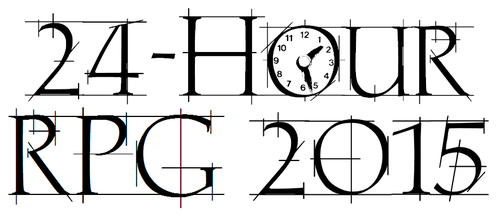
\includegraphics{./images/24hour.png}
\end{document}








